%*******************************************************************************
%*********************************** Second Chapter *****************************
%*******************************************************************************

\chapter{Review of Related Literature}  %Title of the Second Chapter

%********************************** %First Section  **************************************
\section{Crime} %Section - 2.1
    The formal definition of crime varies widely among criminologists but Edwin Sutherland’s short one may be sufficient. According to him, crime is “[a]n unlawful act is not defined as criminal by the fact that it is punished, but by the fact that it is punishable.” \citep{brown2010criminology} But what is punishable may be relative to what the crime is and where it happened. As Sutherland continued, an act can be considered crime in its essence once the State as which the jurisdiction of the act prevails deems such act as an injury and punishable by law.

    In the Philippines, as per the Philippine National Police, crimes can be classified into two: index crimes and non-index crimes \citep{senate2013criminal}. Index crimes are crimes that involve victims such as murder, homicide, physical injury and rape; or against property such as robbery, theft, and burglary. On the other hand, non-index crimes are violations of special laws such as illegal logging or local ordinances. In the Philippines, these classifications are used for statistical purposes and to create a standardized definition of crime classification\citep{tumulak2015crime}.

%********************************** %Second Section  **************************************
\section{Crime Prediction Techniques} %Section - 2.2
    In order to alleviate crime, criminologists are seeking techniques and methods in criminal statistics and analysis to help them prevent and approach crimes better. Machine learning techniques geared towards crime modeling and prediction have already been helping police officials and criminologist in dealing with criminal behaviors.

    A study entitled “Spatio-Temporal Crime Prediction Model Based on Analysis of Crime Clusters” \citep{polat2007spatio} aims to prevent and reduce crime and manage security resources efficiently by forecasting crime. The study area is the Çankaya district of Ankara, the capital city of Turkey. The data used in the study included the number, address, occurrence time, location and type of crime – murder, usurp, burglary, auto related crimes and pickpocketing. Other data such as landmarks and land-use were also included. In the study, clusters are generated and compared with respect to land-use, algorithm, covered area, and suitability to a spatio-temporal crime prediction model. The clustering algorithms to be compared were K-means, Nnh hierarchical, Spatio-temporal Analysis of Crime (STAC), fuzzy, ISODATA, and Geographical Analysis Machine (GAM). The study also aims to determine the most suitable distance metric in implementing clustering. The distance metrics in concern are Euclidean distance and Manhattan distance. After implementing all clustering algorithms, it was found out that K-means, fuzzy and ISODATA can cover all observations in the study area but are spatially inefficient and has difficulty to detect dense crime areas. It was also found that the Nearest neighbor hierarchical approach is not meaningful, is ineffective, and yields too many and too small clusters. The best algorithm was STAC, which showed dense crime areas and covers most area. It includes more homogeneous areas than other methods and indicates denser crime areas than other methods. It is also computationally efficient. As for the distance metric, the Manhattan distance clusters has lower surface area than Euclidean distance clusters. The spatio-temporal crime prediction model had a mean root square error of 1.08 and 1.48 for Manhattan and Euclidean distance applications, respectively. The study recommends to investigate other clustering algorithms to apply the research to another study area.

    Another study called “Modeling and Mapping Crime in Eastern Nairobi, Kenya” \citep{mburu2014modeling} also aims in geospatial crime mapping but this time in Nairobi, Kenya. The study uses a dataset of 1,422 solved crimes constituting 346 series of 10 different crime types. It has three phases: criminal geographic profiling, space and time crime surveillance and future crime prediction. Criminal geographic profiling is a search priority strategy that analyzes the locations of already known crimes in order to predict the residence (or other anchor point) of a serial offender. Space and time crime surveillance is a mixture of time series analysis with kernel density estimation and the space-time permutation scan statistic to monitor patterns over a period of time. Lastly, future crime prediction uses regression analysis to model the relationship between the socio-economic factors in the study area and crime events. The different phases yield different ways to predict criminal activities. Criminal geographic profiling produces a probability surface of crime occurrence. The space and time crime surveillance identifies of crime clusters in space and time, and subsequently identifies of early crime-detection surveillance. Lastly, future crime prediction identifies patterns that will enable prediction of future crime levels.

    Social media can also be important instruments in predicting crime. A study called “Predicting Crime Using Twitter and Kernel Density Estimation” \citep{gerber2014predicting} aims to utilize social media, particularly Twitter, to predict local criminal activity. The study used criminal records from the Chicago Police Department. Tweets tagged with GPS coordinates falling within the city limits of Chicago, Illinois were collected. The criminal records and the tweets are within the same time period. The study uses a two-dimensional spatial probability density function (kernel density estimation) to a historical crime record. The tweets were first tokenized and tagged and were run through the MALLET toolkit to output probable topics. The KDE was then used to map criminal activities extracted as topics from gathered tweets. A surveillance plot measures the percentage of true T crimes during the prediction window (y-axis) that occur within the x\% most threatened area according to the model's prediction for T and it was shown that addition of Twitter-derived features improves prediction performance for 19 of 25 crime types.

\section{Deep Learning}
    Deep learning is a relatively new field of machine learning \citep{deng2014deep}. It is defined to be a set of techniques that employ multiple layers of non-linear information processing for feature extraction and transformation, and for pattern analysis and classification. These techniques have already been used for a wide range of signal and information processing work. Deep learning has gained popularity due to improved computational capabilities of chips (graphic processing units or GPUs), the emergence of big data and recent advancements in machine learning research. One of the most successful deep learning techniques is the Long Shot-term Memory (LSTM) network \citep{schmidhuber2015deep}, a kind of Recurrent Neural Network (RNN).

\section{Recurrent Neural Networks}
    Neural networks are one of the most popular machine learning method \citep{razi2005comparative}. They are effective because of their ability to predict complicated nonlinear relations from the input data, model disjoint decisions with random shapes and to determine unknown classes \citep{huang2006real}. But despite their success, traditional neural networks are still faced with the incapacity to predict patterns in time and allow persistence of information \citep{patan2008artificial}. Ironically, neural networks were designed to emulate the connections of the neurons in our brain to model decisions but unlike neural networks, human thoughts have persistence. We derive our decisions by accumulating experience and using them as factors in calculating outcomes and making judgements. A factor may be heavier in one decision than another. Different situations demand different weighing of experience. Our decisions are not just affected by the situation itself but from our previous decisions. Unfortunately, traditional neural networks does not allow persistence of information to have effect on its future predictions.

    \begin{figure}[H]
    \centering
    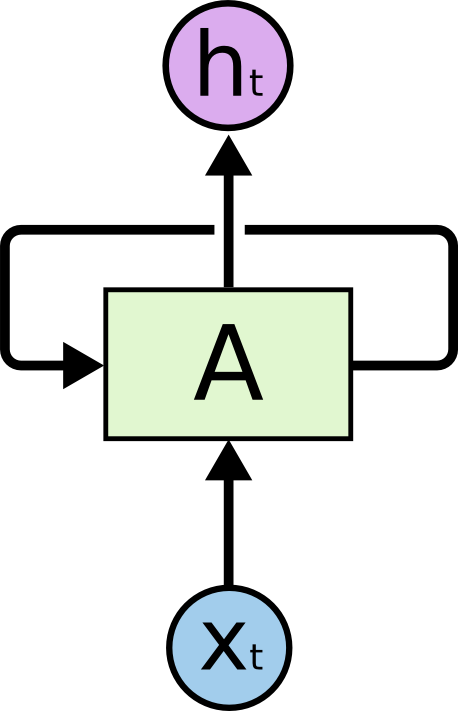
\includegraphics[width=2cm]{RNN-rolled}
    \caption{An illustration of a recurrent neural network \citep{olah2015understanding}}
    \end{figure}
    Recurrent neural networks (RNN) solve this predicament. As shown in Figure 2.1, these networks have loops in them that carries persistent information \citep{mikolov2010recurrent}. In traditional neural networks, hidden neurons have weighted connections only to the outputs. In RNNs, in addition to a feed to the output, a hidden neuron has a weighted connection to the hidden layers of the next time step, represented as a loop to itself. This connection represents the persistence of data throughout the timesteps/iterations of data in the network.

    \begin{figure}[H]
    \centering
    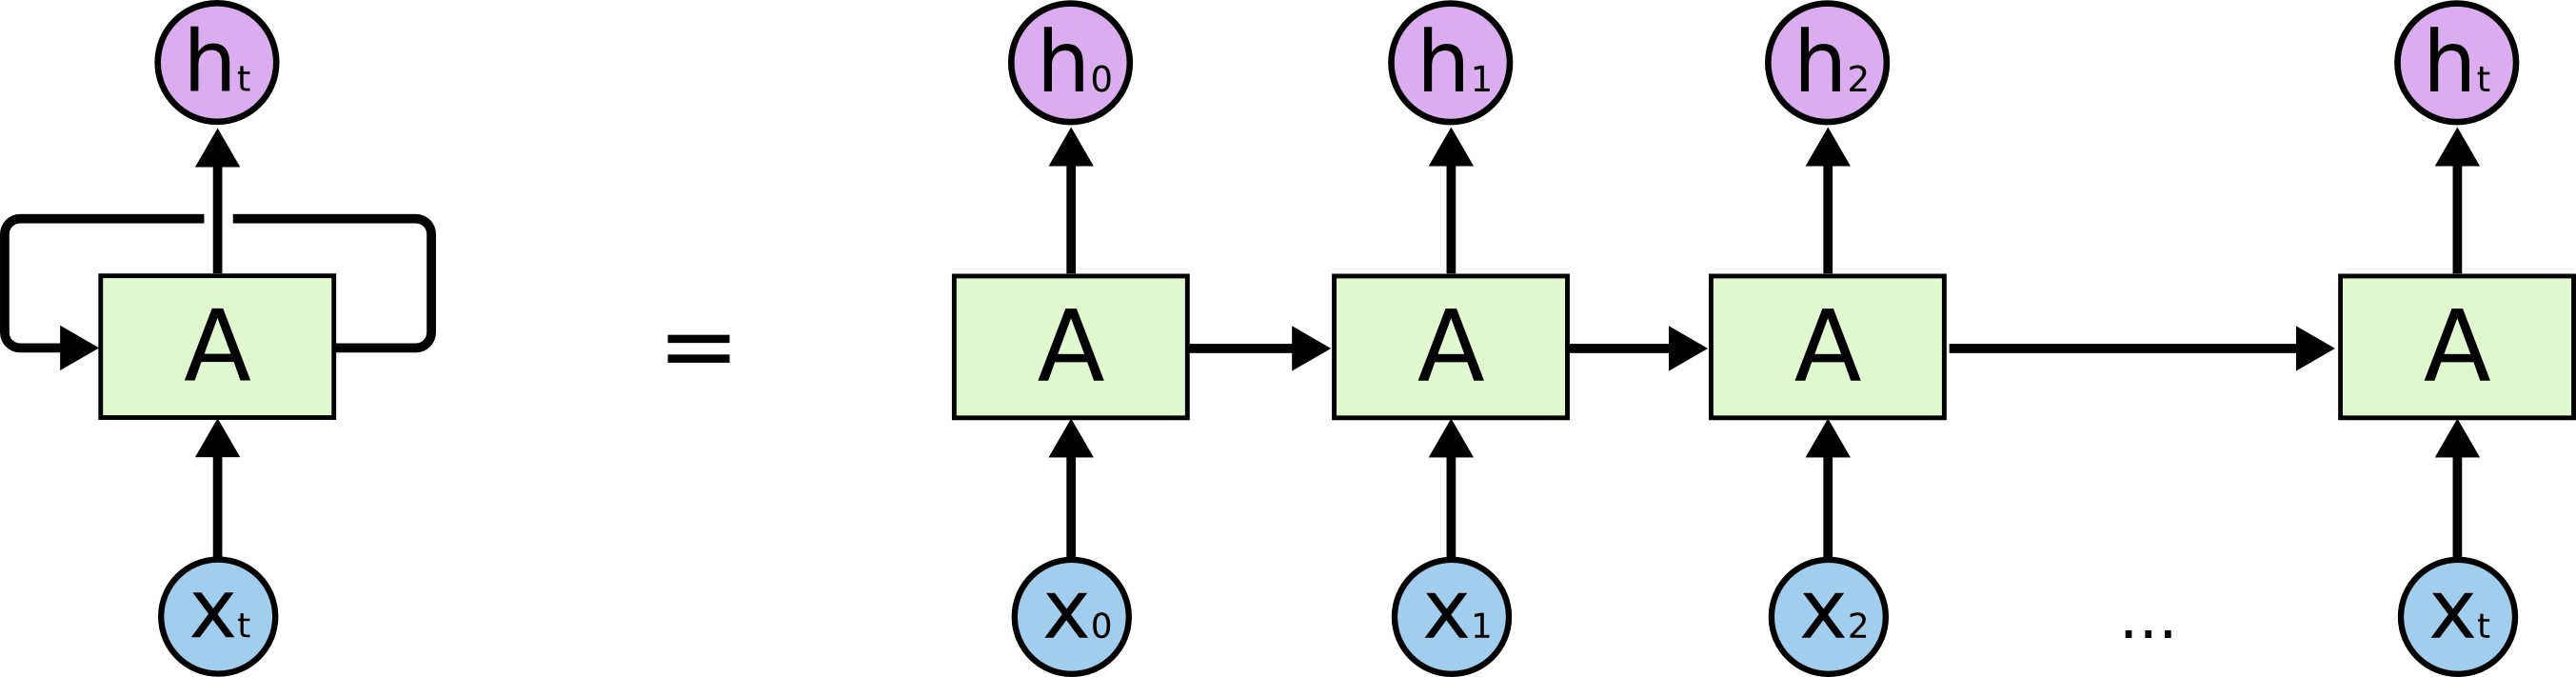
\includegraphics[width=12cm]{RNN-unrolled}
    \caption{An unrolled recurrent neural network \citep{olah2015understanding}}
    \end{figure}
    Figure 2.2 shows a recurrent neural network with its loops unrolled. The chain-like structure it illustrates hints that recurrent neural networks are related with sequences and lists. RNNs have been effective for a wide range of problems that deals with a series of data including speech recognition, image processing and language modeling \citep{olah2015understanding}.

    RNNs are useful in representing the history and memory but it has some setbacks as well. They might have the ability to create memory from previous information but they have a hard time connecting information as the gap between a relevant information and the point where it is important grows \citep{graves2012supervised}. This is called the Long-term Dependency Problem \citep{bengio1994learning}. To solve this problem, an architecture of RNN was introduced, the Long Short-Term Memory or LSTM.

\section{Long Short-term Memory Networks}
    Long Short-term Memory Networks (LSTMs) are a special type of RNN that gracefully deals with the long-term dependency problem \citep{hochreiter1997long}. They are capable of remembering data over long period of time by implementing a more complicated structure in its repeating module.

    \begin{figure}[H]
    \centering
    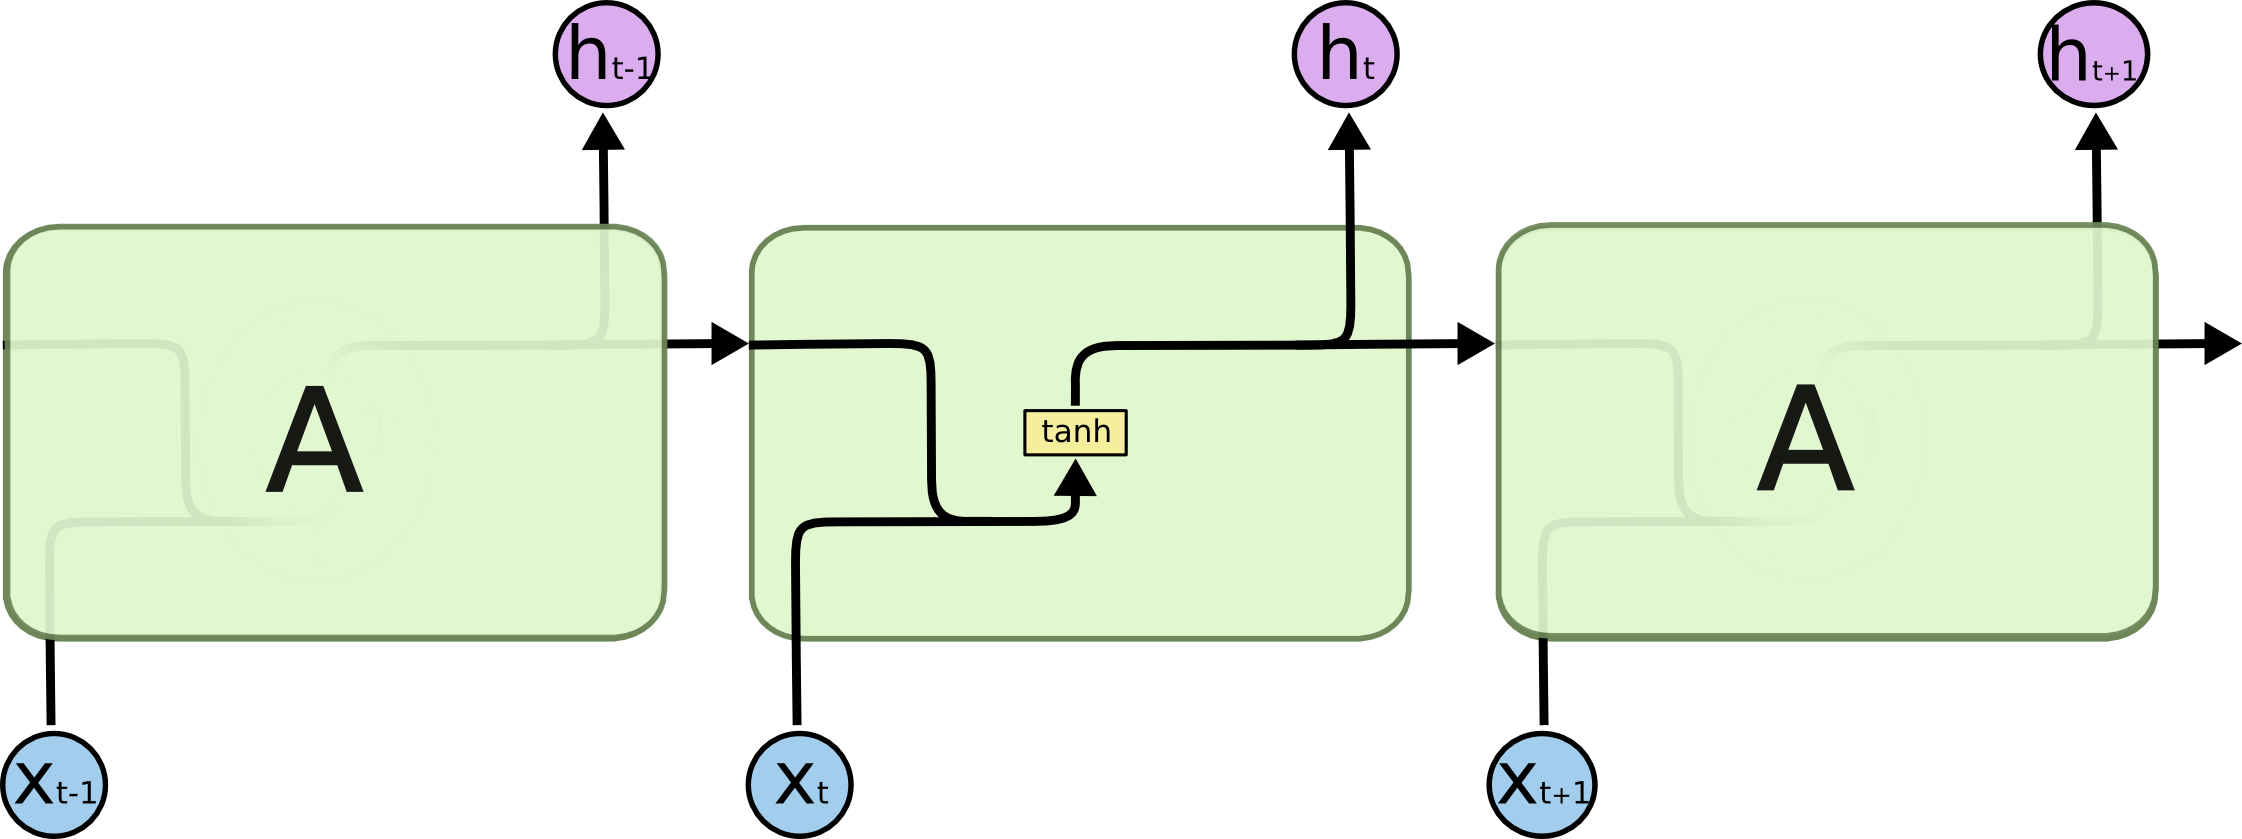
\includegraphics[width=12cm]{LSTM3-SimpleRNN}
    \caption{A traditional recurrent neural network has a single layer \citep{olah2015understanding}}
    \end{figure}
    Traditional RNNs have simple recurring layers. Figure 2.3 shows an example of an RNN with a tanh layer in its repeating module. In this network, the current input and the output of the previous layer will be fed to a tanh activation equation and the result will be the output for that layer.
    
    \begin{figure}[H]
    \centering
    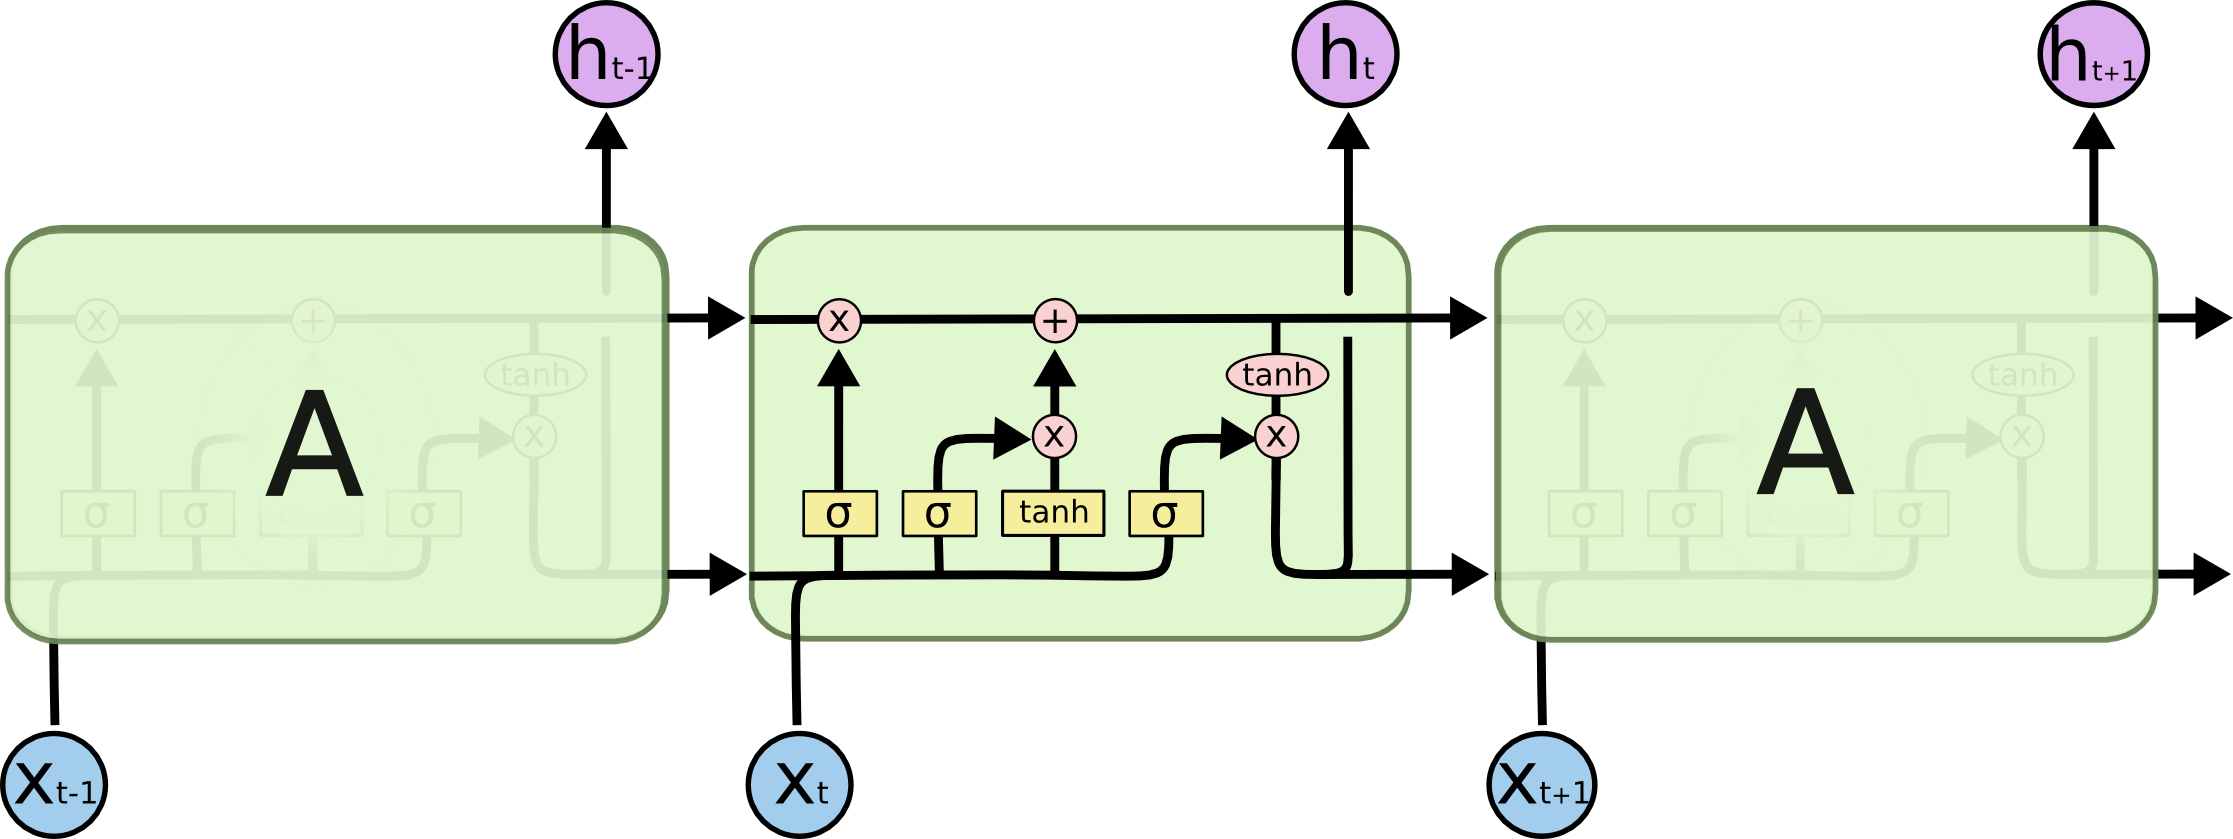
\includegraphics[width=12cm]{LSTM3-chain}
    \caption{An LSTM layer \citep{olah2015understanding}}
    \end{figure}
    LSTMs, on the other hand, use a different structure that employs four activation layers. Figure 2.4 illustrates how these layers interact with one another. The next section will elaborately explain the operations and elements involved in an LSTM layer.

\section{LSTM Structure}
    This section will walk through the structure and mechanics of an LSTM layer. The figures that will follow will refer to these expressions.
        \begin{itemize}
        \item \( x_t \): Input for the current layer
        \item \( h_{t-1} \): Output of the previous layer
        \item \( h_t \): Output of the current layer
        \item \( C_{t-1} \): Cell state of the previous layer
        \item \( C_t \): Cell state of the current layer
        \end{itemize}

    \subsection{Cell State}
        \begin{figure}[H]
        \centering
        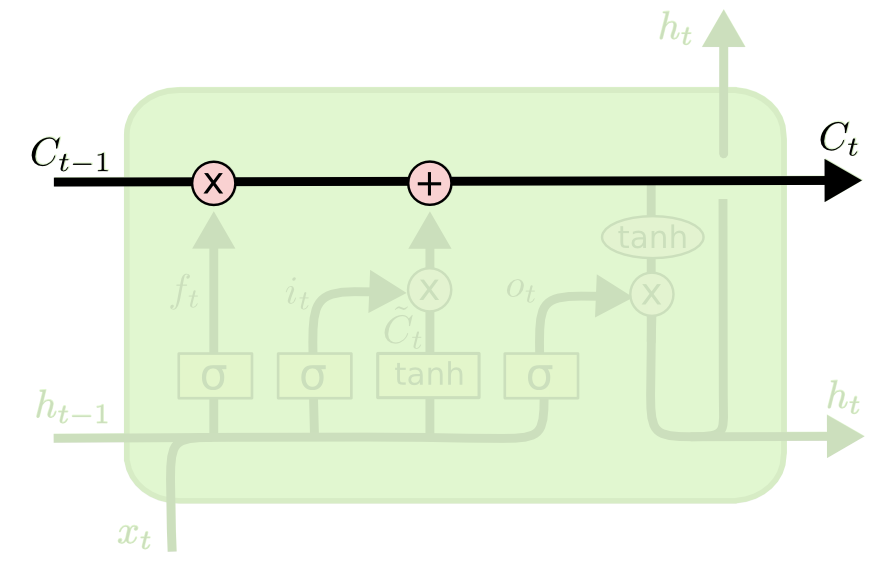
\includegraphics[width=14cm]{LSTM3-C-line}
        \caption{The Cell State \citep{olah2015understanding}}
        \end{figure}
        The core idea of LSTMs is to protect and control the cell state. As shown in Figure 2.5, the cell state is like a line traversing through the layers of the network. It holds the information from the previous layers it has passed through. The cell state and the input of the current layer determines the output for that layer. The amount of information that the cell state will carry from the previous layers is determined by a set of interacting gates.

        \begin{figure}[H]
        \centering
        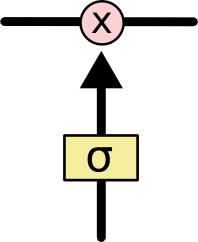
\includegraphics[width=2cm]{LSTM3-gate}
        \caption{A gate in LSTM \citep{olah2015understanding}}
        \end{figure}
        Gates control how much of the information will pass through to the next layer in the cell state. It is made up of a sigmoid neural net layer and a multiplication operation, as shown in Figure 2.6. The sigmoid layer will have a value between zero or one, indicating how much of the current cell state will be let through. Zero multiplied with the current cell state will always be zero so this means that nothing will be let through. One, on the other hand, means everything will be let through.

        The next parts will explain the three gates in a standard LSTM.

    \subsection{Forget Gate}
        \begin{figure}[H]
        \centering
        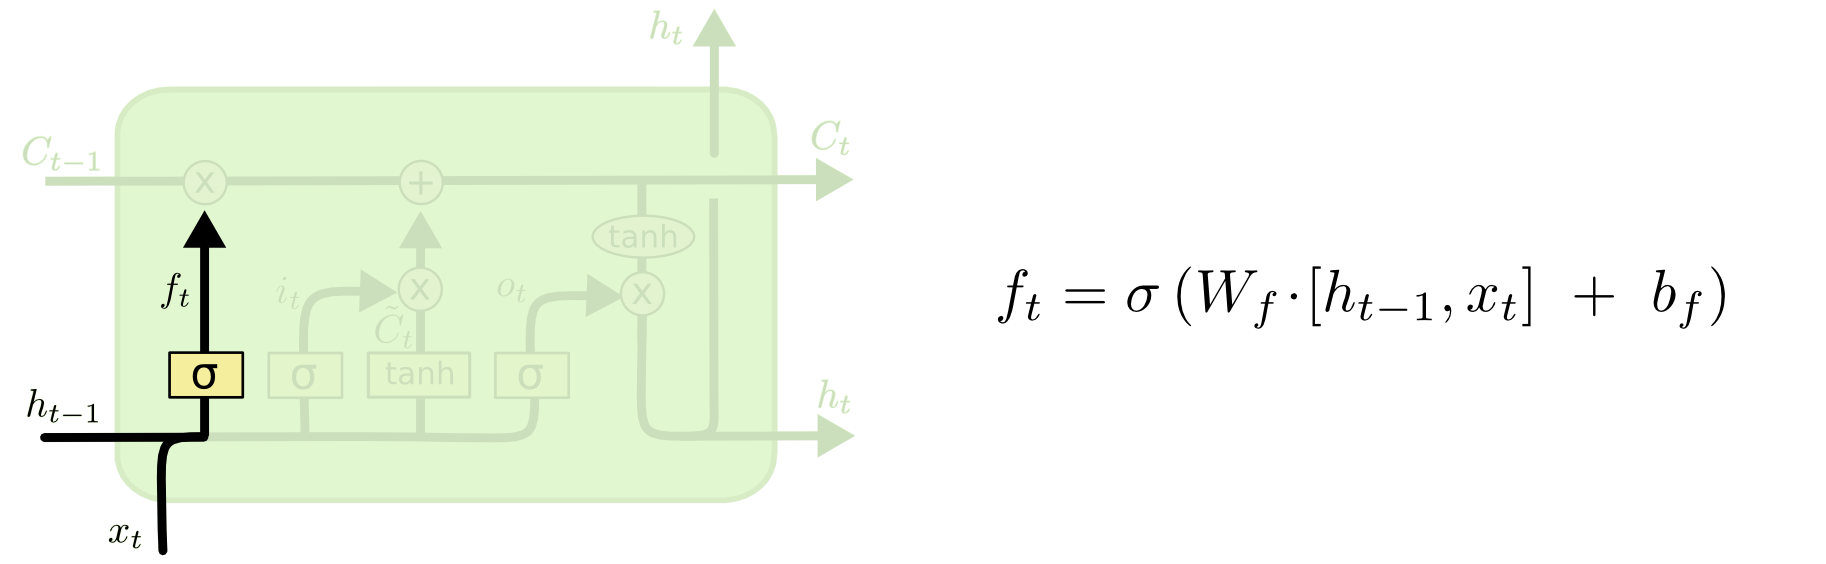
\includegraphics[width=8cm]{LSTM3-focus-f}
        \caption{The forget gate in LSTM \citep{olah2015understanding}}
        \end{figure}
        The first gate in the LSTM is called the forget gate. This gate decides how much of the input of the current layer and the output of the previous layer will be forgotten. Figure 2.7 shows the structure of this gate and the corresponding equation. For instance, in a language model that will check for correct pronouns (e.g. his or her), the gender of the subjects in the previous sentences will be forgotten when a new subject is encountered.

    \subsection{Input Gate}
        The next gate in the LSTM is the input gate. This gate updates the old cell state \( C_{t-1} \) to a new cell state \( C_t \). This gate has two parts.

        \begin{figure}[H]
        \centering
        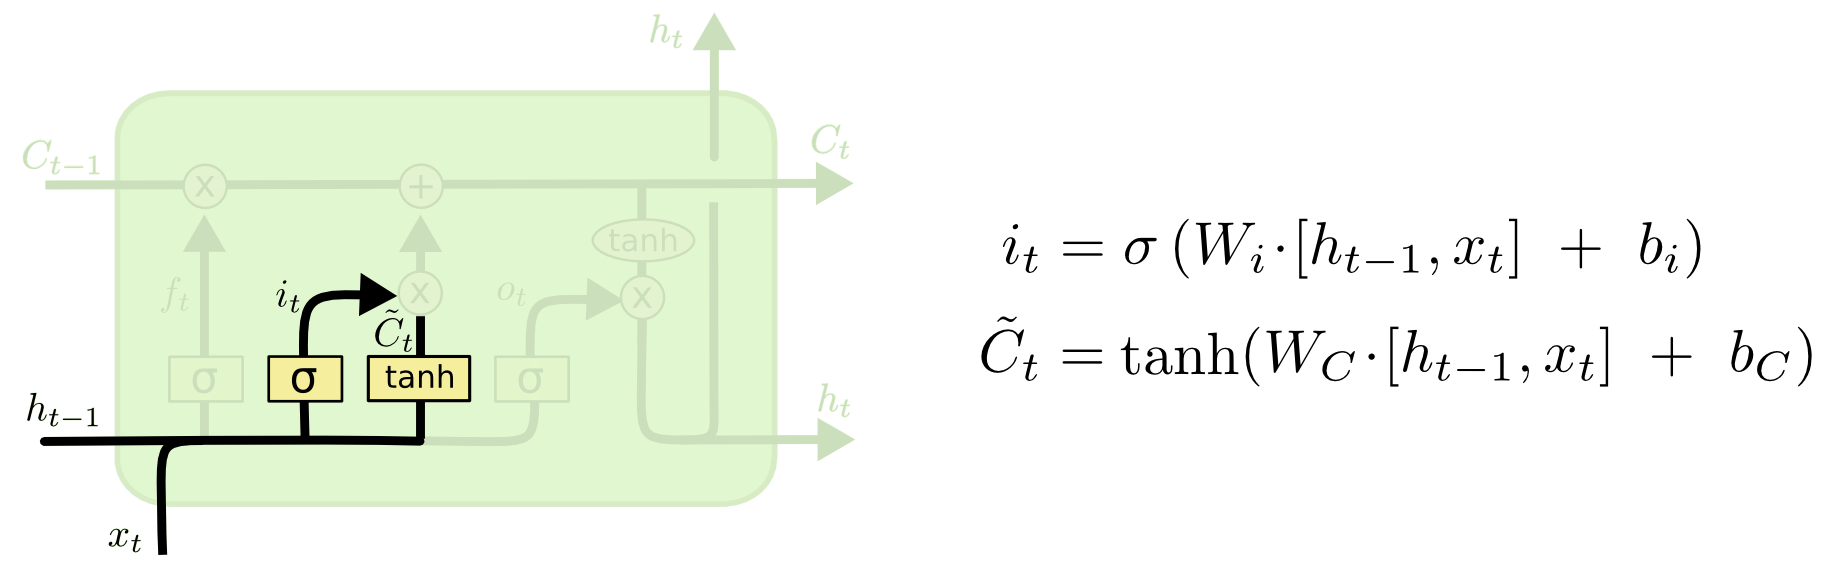
\includegraphics[width=8cm]{LSTM3-focus-i}
        \caption{The input gate in LSTM \citep{olah2015understanding}}
        \end{figure}
        The first part is a sigmoid layer \( i_t \) that decides the values that will be updated. Next is a tanh layer \(\tilde{C}_t\) that will add new values to cell state. Figure 2.8 shows these two parts.

        \begin{figure}[H]
        \centering
        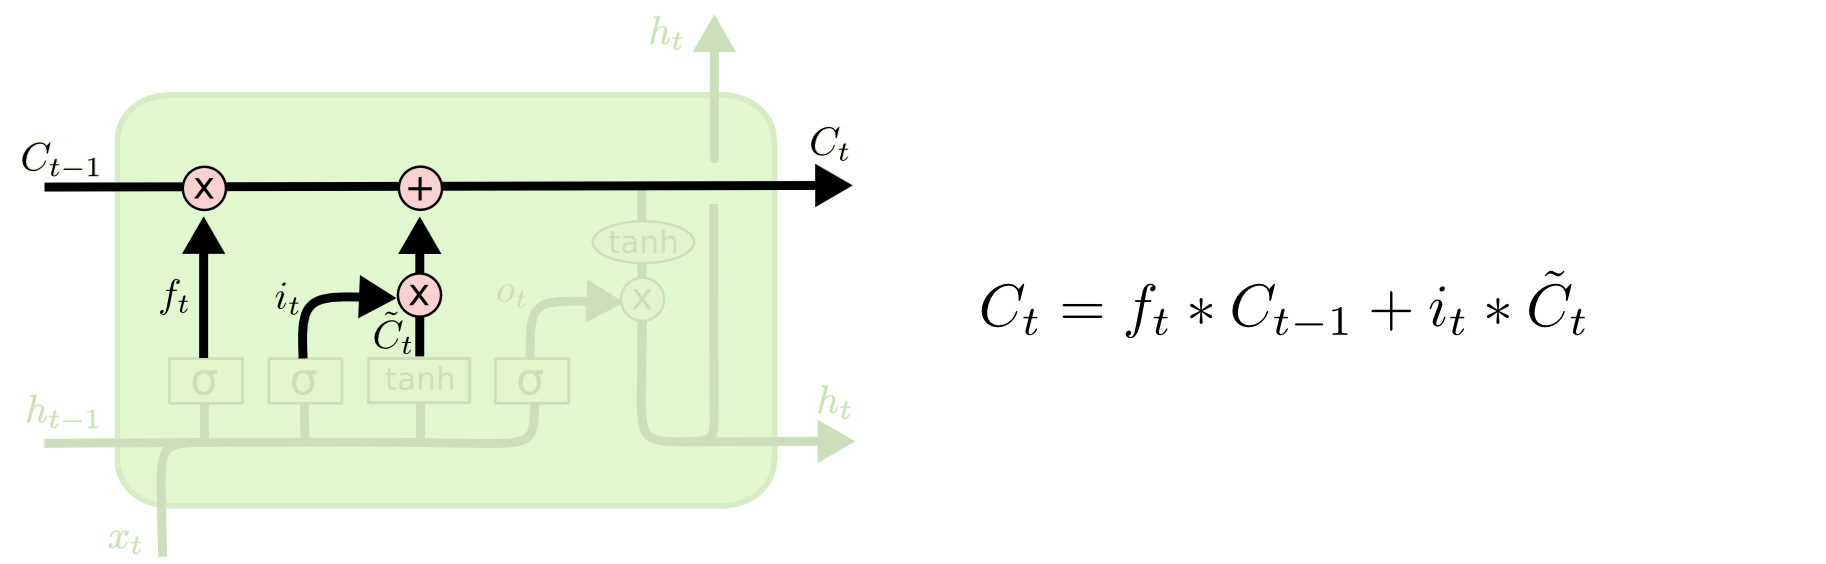
\includegraphics[width=8cm]{LSTM3-focus-C}
        \caption{Cell state update \citep{olah2015understanding}}
        \end{figure}
        After the input gate, the cell state will be updated with the values of the forget gate and input gate. In our language model example, this is the point where the previous gender of the subject is actually dumped and is updated with the gender of the new subject.

    \subsection{Output Gate}
        \begin{figure}[H]
        \centering
        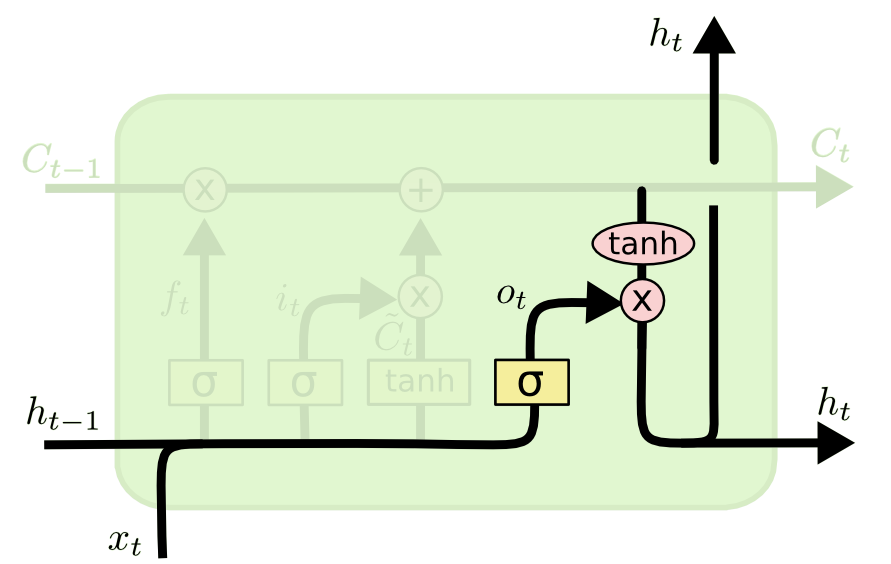
\includegraphics[width=8cm]{LSTM3-focus-o}
        \caption{The output gate in LSTM \citep{olah2015understanding}}
        \end{figure}
        The last part of the LSTM will determine the output to the next layer. The cell state is fed through a tanh layer and then multiplied with a sigmoid layer. The sigmoid layer is similar to the forget gate but instead of determining how much we want to forget the current input and previous output, this layer will determine how much we want to remember. Multiplying it with the tanh layer will result to the parts that we want to output. This will result to a filtered version of the cell state. In our language model example, plurality of the new subject or the tense of the subject's action could be added in order to correctly check the proper pronoun.

\section{Crime Recurrence}
    \begin{figure}[H]
        \centering
        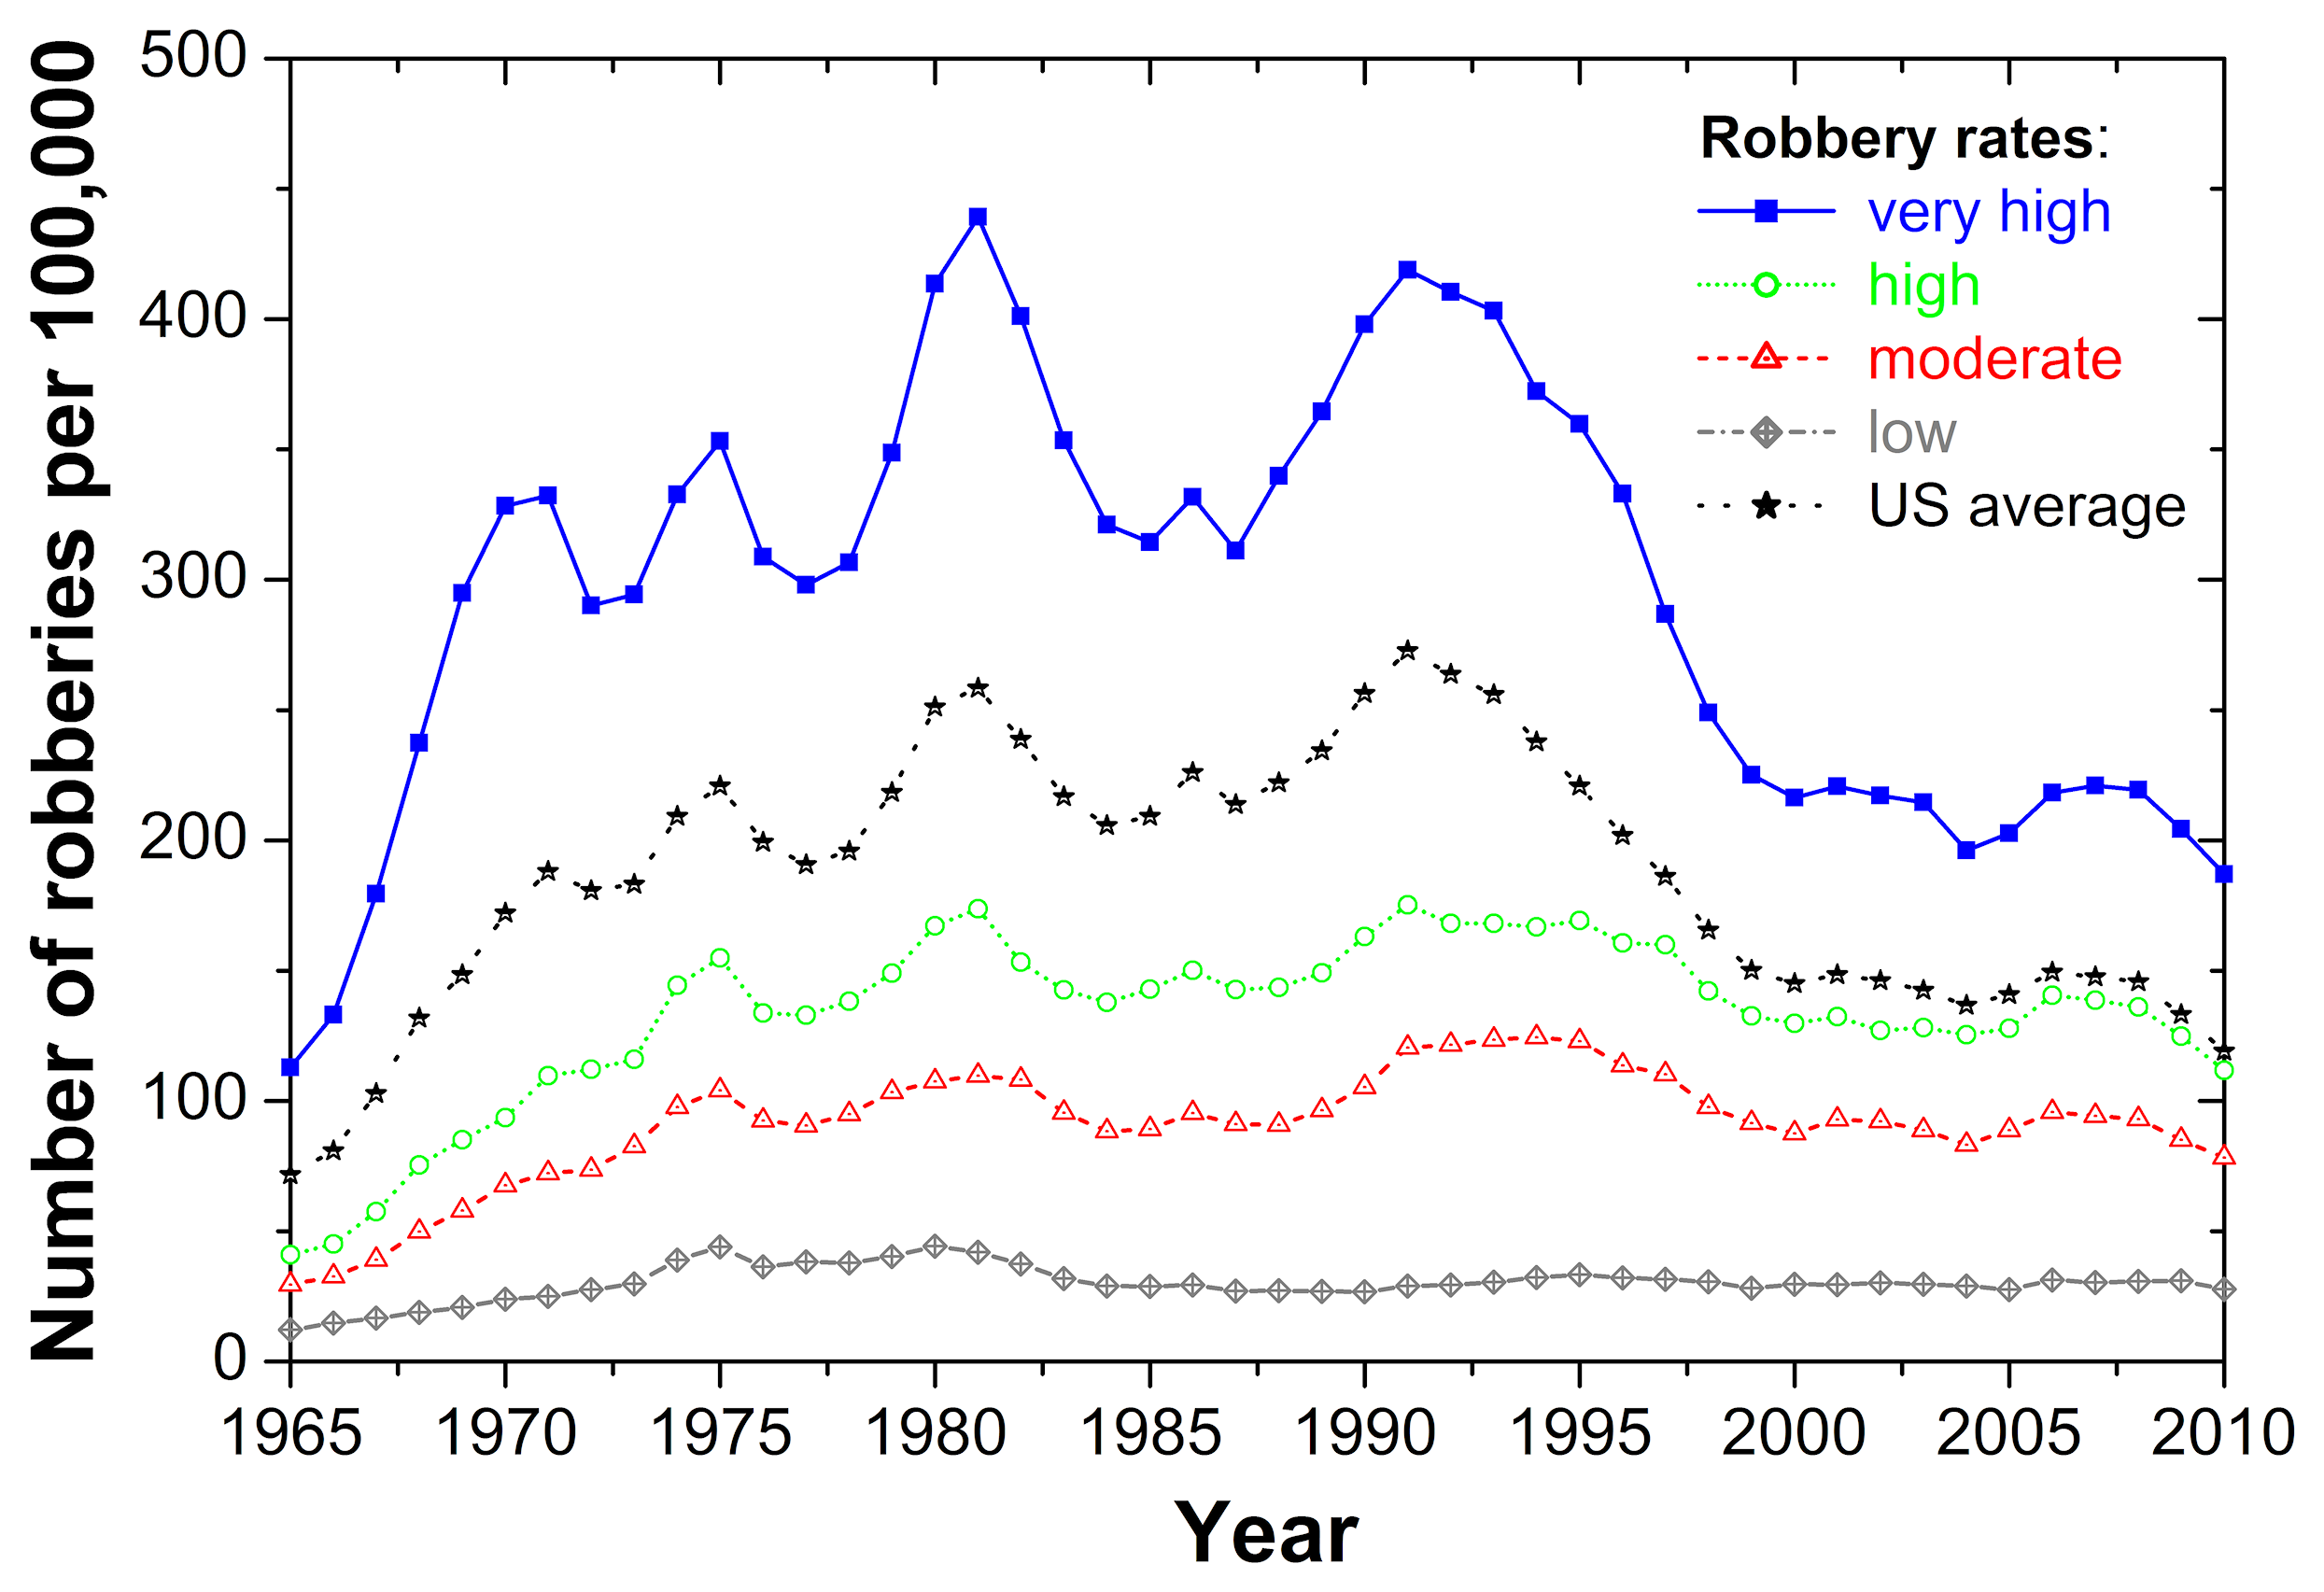
\includegraphics[width=12cm]{crime-recurrence}
        \caption{Empirical evidence for the recurrent nature of crime \citep{perc2013understanding}}
    \end{figure}
    Crime may all seem random at first glance but according to \cite{perc2013understanding} in their 2013 study entitled \textit{Understanding Recurrent Crime as System-Immanent Collective Behavior}, crime exhibits a recurrent nature. Empirical data shown in Figure 2.11 illustrates this behavior of crime. Along with the US average (black line), the different lines in the graph represents the different categories of US states according to average rate of robberies. US states were categorized into very high (blue), high (green), moderate (red) and low (gray) robbery rate groups. The values of these lines are the average crime rates of the different categories from 1965 to 2010. The blue line, or the average robbery rate of US states with very high robbery rate, significantly oscillates over time, suggesting a recurrent behavior. The same trend can be noticed for the US average and in categories with high and moderate robbery rate but they have lesser intensity. States with low robbery rate have a much more stable average robbery rates. The same behavior can be seen on other kinds of crime like motor vehicle theft and property crime. This data proves that crime is recurrent in nature regardless of type and intensity.